\chapter{Stand van zaken}
\label{ch:stand-van-zaken}

Bij dit hoofdstuk wordt de literatuurstudie besproken. Qua literatuur is er gezocht naar info die te maken heeft met de 3 grote pijlers van dit onderzoek. Eerst wordt besproken wat de literatuur vermeldt over studenten aan een hogeschool en hun gedrag. Vervolgens bekijkt men wat de devices zijn die studenten meebrengen naar school en welk effect ze mogelijks kunnen hebben. Als laatste wordt gekeken naar de resultaten die studenten behalen en de mogelijke oorzaken/gevolgen.

\textcite{Johnson2017} onderzochten hoe academisch de smartphone werd gebruikt bij studenten van een business-school. Hoewel hun onderzoek niet statistisch volledig significant was, konden zij toch concluderen dat smartphones een impact hadden op de studenten, soms positief, soms negatief. Positief was bijvoorbeeld de mogelijkheid om voor elk probleem dat de student tegenkwam bij schooltaken een applicatie te downloaden op hun smartphone die het probleem deels vor hem kon oplossen. Ook heeft de komst van de laptops ervoor gezorgd dat studenten hun taken zorgvuldiger en beter op tijd kunnen afronden. Zij merkten ook in hun onderzoek dat het bezit van een smartphone of ander elektronisch device een boost gaf aan hun ego of imago in de klas. Negatief voor de studenten was dat de apparaten voor afleiding zorgen en als gevolg daarvan de punten lager zijn. \textcite{Hossain2016} hun onderzoek sluit hierbij aan. Zij vonden dat onder 316 studenten ongeveer 2/3 van de studenten hun smartphone gebruikten om academische informatie op te zoeken. 

Deze bovenstaande onderzoeken duiden aan dat studenten wel degelijk hun devices voor schooldoeleinden gebruiken en dit ook zelf duidelijk aangeven. Ze kunnen gemakkelijker samenvattingen schrijven, sneller een vraag stellen aan medestudenten… Toch blijft de vraag hoeveel tijd er werkelijk besteed wordt aan deze schooltaken, en hoeveel tijd er gaat naar ontspanning op de smartphone. Hier wil het onderzoek in een later stadium een beter antwoord op geven.

\textcite{Alfawareh2014} keken naar het aantal studenten van een universiteit in Saudi-Arabië dat een smartphone meenam naar school. Zij vonden dat wel 94,4 procent van de ondervraagden in het bezit was van een smartphone. Het is dus ook te verwachten in de resultaten van dit onderzoek dat meer dan 95 procent van de ondervraagden een of ander elektronisch apparaat altijd meenemen naar de les. 91,69 procent gebruikten hun smartphone om in te loggen op het portaal van de universiteit. Opvallendste voor dit onderzoek is dat uit hun resultaten bleek dat maar 54,49 procent van de ondervraagde personen hun smartphone altijd of soms gebruikte om klasmateriaal (slides, pdf’s, nota’s) te downloaden of te gebruiken voor een les. Gebruik van laptops werd hier niet onderzocht. Het Student Mobile Device Survey \autocite{Harris2015} heeft wel gekeken naar het gebruik van laptops. Zij vonden in hun onlineonderzoek in de Verenigde Staten dat verspreid werd onder 1211 hogeschoolstudenten tussen de 18-30 jaar dat 87 procent van de hogeschoolstudenten hun laptop elke week gebruiken voor schoolwerk, terwijl maar 64 procent gebruik maakt van hun smartphone hiervoor en maar 40 procent een tablet gebruikt. Hieruit blijkt dus dat smartphones minder worden gebruikt voor schooldoeleinden dan laptops. Smartphones dienen bij de studenten meer als verzetje en ontspanning, waar meer studenten hun laptop bovenhalen voor schooltaken uit te voeren of te leren.

\textcite{Lee2014} hadden naar aanleiding van klachten van scholen (slaaptekort bij studenten, tekort aan aandacht tijdens lessen…) hun onderzoek gericht op de smartphone die mogelijks de boosdoener was. Waar andere onderzoeken meer een toelichting gaven van wat de student doet op de smartphone, gingen zijn via zelfontwikkelde software binnendringen in 95 studenten hun smartphone en data binnenhalen over het gebruik van de smartphone. Zij verdeelden 95 studenten in 2 groepen op basis van studieresultaten. Zo konden zij achterhalen dat groep met lagere punten 50 minuten per dag langer hun smartphones gebruikten dan de betere studenten. Dit onderzoek zet aan om in de resultaten van de enquête na te gaan of de studenten met schoolresultaten boven het gemiddelde inderdaad minder tijd spenderen achter hun smartphone.
Volgens een ouder onderzoek \autocite{Morahan-Martin1999} heeft het soms ziekelijk gebruik van de smartphone een onderliggend probleem, meestal op sociaal of mentaal vlak. Het mag dan ook geen toeval meer noemen dat het veelvuldig gebruik van smartphones in 2013 erkend is als een gedragsstoornis door de medische wereld.  

We mogen nu veronderstellen op basis van vorige bronnen, dat bijna elke student een elektronisch device meeheeft, en dat het vaker een negatief effect met zich meebracht dan een positief effect op de student die in de les zit. Mogelijks heeft het studeren met een laptop wel een positiever effect dan zonder. Toch is de logische vraag natuurlijk of het niet beter is voor de student om de toestellen op een correcte manier de student aan te bevelen om dit apparaat niet meer te gebruiken tijdens de lessen/schooluren.

\textcite{Beland2016} keken daarom in hun onderzoek wat de impact zou zijn voor het verbannen van smartphones op de resultaten van de student. Hiervoor gingen ze langs op 4 verschillende scholen in Engeland. Zij kwamen uit dat tussen de testscores van voor de ban op smartphones en erna een verschil zat van 6,41 procent qua standaarddeviatie. Zij gaven aan dat het grote verschil in prestaties van de studenten geleid werd door een grote positieve invloed van het bannen op de studenten die zeer laag scoorden voor de verbanning van de smartphone. Na het verbannen bleken zijn veel positievere resultaten te behalen dan ervoor. Daarnaast concludeerden ze ook zoals vorige onderzoeken dat deze apparaten een negatieve impact hebben door het bieden van afleiding aan de student. Zeer interessant was bij hun onderzoek dat bij de studenten die normaliter lage punten scoren, zelfs een verschil in testscores te merken was van 14,23 procent qua standaarddeviatie. Je kan hieruit concluderen dat studenten met hoge punten mogelijks beter kunnen omgaan met de afleiding die een device biedt dan studenten die minder aandacht schenken aan de kwaliteit en score van hun resultaten. Dit onderzoek toont aan dat we in onze resultaten verder moeten kijken naar de studenten die lager dan het gemiddelde scoren, en kijken of zij misschien gebaat zijn bij een ban, en of ze zelf positief staan ten opzichte van een verbanning van smartphones op school.

\textcite{Farley2015} keken in Australië naar de mogelijkheden die smartphones kunnen bieden binnen het klaslokaal, of aan het bureau van de student. In 2013 hadden zij reeds onderzoek gedaan naar de gevolgen voor scholen wanneer ze e-learning volledig zouden omarmen. Dit zou niet alleen veranderingen meebrengen voor de volledige infrastructuur van een school, maar ook aan de manier van lesgeven. Het concept BYOD (Bring your own device) kan zowel de student als de school helpen in het groeien naar e-learning: Scholen hoeven geen extreme kosten te doen aan hardware-voorzieningen, en studenten kunnen altijd en overal leren via hun mobiel apparaat. Volgens \textcite{Crompton2014} staan ook vele leerkrachten niet te springen voor het overschakelen naar lessen waarin gebruikt gemaakt wordt van technologie uit de 21ste eeuw. Leerkrachten zouden hiervoor hun stijl van lesgeven moeten aanpassen. \textcite{Farley2015} keken naar 749 studenten bij hun online enquête. Zij vonden allereerst dat studenten die een hogere opleiding volgen vaak meer dan 1 device met zich meebrengen naar de les. 90 procent van hun testpubliek gaf aan dat ze de laptop gebruikten om hun studies te ondersteunen, terwijl 73 procent ook hun smartphone gebruiken voor hun studies. 

De onderzoeken in bovenstaande alinea worden vooral aangehaald om te tonen dat er manieren zijn om de afleiding die laptops en smartphones bieden aan studenten de kop in te drukken, maar dat men ze nog niet optimaal gebruikt. Zolang men deze apparaten niet gaat omarmen als vrienden tijdens de les zal er ook geen mogelijkheid zijn om veranderingen te zien aan het gedrag dat studenten vertonen tijdens de les. Als de studenten verplicht worden om hun apparaten intensief te gebruiken voor meer dan 75 procent van het lesuur, zal de afleiding dalen en de leergierigheid en het optimisme alsmaar stijgen. In bovenstaand onderzoek van \textcite{Farley2015} gaven de studenten zelf aan dat PowerPoint-slides of forums vaak voorkomen tijdens lessen terwijl podcasts, virtuele klassen of opgenomen lessen maar zelden worden gebruikt als mogelijks studiemateriaal voor de student. 85 procent van de studenten gaf zelfs aan dat een vooraf opgenomen les aangevuld met slides een verbetering zou bieden van de motivatie om te studeren.

Als laatste deel in dit hoofdstuk bespreken we ook kort beide scholen die zijn opgenomen in de steekproef.

Hier begin ik aan zodra ik antwoord krijg van enkele vragen gericht aan meneer Denis Amelynck!

\section{HoGent, Gent, België}
\label{sec:hogent}

\section{De Haagse Hogeschool, Den Haag, Nederland}
\label{sec:haagsehogeschool}

\begin{figure}
	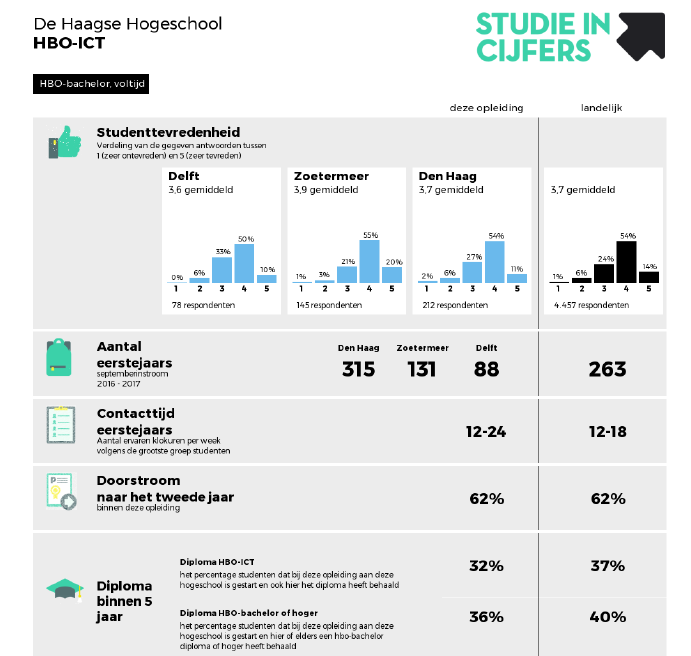
\includegraphics[width=\textwidth]
	{img/hbo-ict.png}
	\caption{Dit is testafbeelding, om te kijken of deze goed gaat werken in de toekomst.}
	\label{fig:hboict}
\end{figure}

In Figuur \ref{fig:hboict} ziet u de resultaten van HBO-ICT, dit als klein testje voor wanneer ik reactie krijg van mr. Amelynck

\section{Vragen voor Onderzoek}
\label{sec:eindliteratuur}

Uit deze studie en alle bovenstaande informatie halen we volgende onderzoeksvragen, die hopelijk beantwoord zullen worden door de resultaten in volgende hoofdstukken:

\begin{itemize}
	\item Heeft het gebruik van smartphones en laptops tijdens de lessen mogelijks een invloed op de slaagcijfers en kennis van de student? (Hoofdvraag)
	\item Heeft geslacht, relatiestatus of leeftijd van de student een invloed op de aantrekkingskracht die deze devices hebben op de student?
	\item Is er een verschil in omgang met devices tussen Nederlandse en Vlaamse studenten?
	\item Wat denken studenten zelf over de invloed van smartphones op hun resultaten?
	\item Is er een verschil in gebruik van smartphones en in resultaten tussen studenten uit een sociale richting en studenten uit een richting die IT-gerelateerd is?
	\item Is er een direct positief effect op de student in het klaslokaal wanneer de smartphone en laptop volledig uit beeld verdwijnen?
\end{itemize}
